\documentclass{article}
\usepackage[utf8]{inputenc}
\usepackage{blindtext}
\usepackage{graphicx}
\usepackage{hyperref}
\usepackage[dvipsnames]{xcolor}

\title{Report: Locating Chinese Districts in Any City}
\author{Nan He}
\date{June 2021}

\begin{document}

\maketitle

\section{Introduction}
\subsection{Background}
More and more Chinese works and study overseas in the United States, Canada, and other western countries in recent decades.
Oversea Chinese population in the US grow from $3,347,229$ in 2010 to $4,143,982$ in 2020.\cite{census2010chi, census2020chi}
The growing presence of these new Chinese workers has a significant impact on existing local Chinese communities in major western cities.
Research suggested that the newcomers help to revitalize and transforming old Chinatown. \cite{jia2010chinatown}
They also boost many non-traditional Chinatowns or "Chinese Districts" in various middle-sized cities where the local Chinese population is small.

For international Chinese students like me, the existence of a local Chinatown or "Chinese districts" is important for residential decisions.
The combination of Authentic Chinese and Asian food, Asian supermarkets, and various services in the Chinese language provides a smooth cultural transition for many newcomers. Previous publications support my personal experiences.\cite{zhou2010chinatown} This report focuses on finding the opportunities inside this trend.

\subsection{Business Problem}
One major problem of the Chinese districts in middle-sized western cities is that their distributions are generally obscure, especially for someone who is not Chinese.
When I visited Charlotte and Atlanta the first time, when discussing which areas have good access to Chinese services and goods, every person almost gave different answers.
Some have already lived there for over five years while still have no clear clue whether a "Chinese District" exists and where it is.
Inspired by these experiences, in this report, I will investigate this problem and try to build a tool to find the location of an existing Chinese District for any given city using a data-driven approach.

\subsection{Significance (Target Audience)}
This problem has values for two types of users. Firstly, investors can identify potential investments in Chinese venues, especially those who are not local to that city or are not familiar with the Chinese communities. Secondly, for other Chinese students and oversee works who seek to find a comfortable environment in an unfamiliar city.

\section{Data}
Two types of data are needed to achieve our goal of finding Chinese districts automatically for a given city or area,

1. Data that tells us what a Chinese district should look like.

2. A target city or area the user wants to investigate.

In the following sections, I will discuss details of data acquisition and cleaning.
Examples of what the data looks like, together with the features extracted are presented below.

\subsection{Chinese District Feature Data}

For data 1, I retrieve the location of 5 large Chinatown in the US from \href{https://en.wikipedia.org/wiki/Chinatowns_in_the_United_States}{\textcolor{blue}{this Wikipedia page}}. 
Note that ten are listed on that page, and many of them cluster on the west coast. So I choose only New York, San Francisco, Los Angeles, Chicago, and Huston, to make the data more balanced geographically.
A good starting point to study what defines a Chinese district is from the venues in that area.
Therefore, to extract venue data for those areas, I utilize the Foursquare API, a popular location service provider based in the US.\cite{foursquare}

The latitudes and longitudes of the five selected Chinatowns are:
\begin{figure}[h]
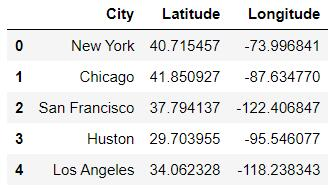
\includegraphics[width=0.5\textwidth]{c1.jpg}
\centering
\end{figure}

Some example resulting venues are:
\begin{figure}[h!]
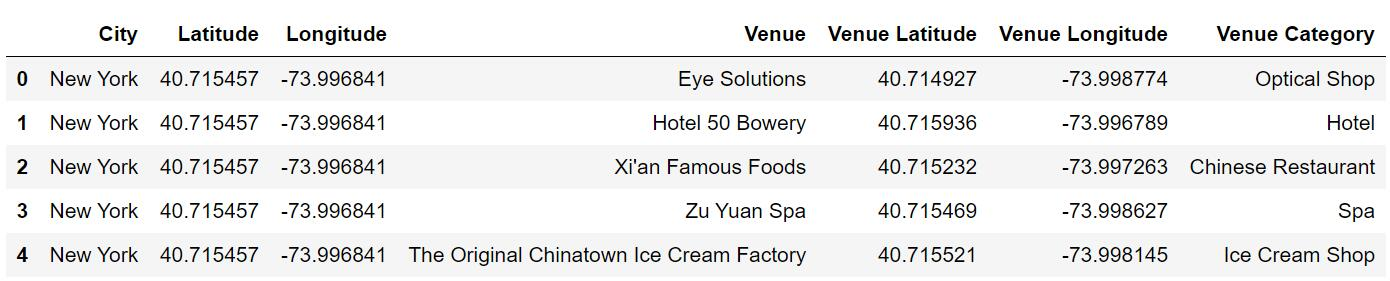
\includegraphics[width=1.0\textwidth]{c2.jpg}
\centering
\end{figure}

In total, 429 venues are selected around these five Chinatowns; those data will tell us what defines a Chinese district.

\newpage

The data will be grouped by the city name and encoded in terms of the venue category. Examples look like:
\begin{figure}[h!]
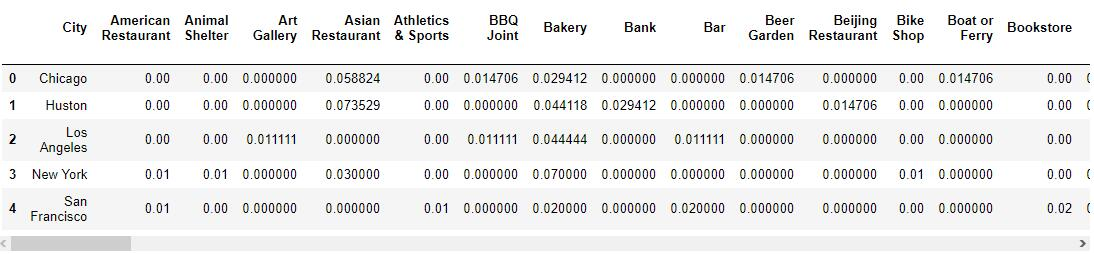
\includegraphics[width=1.0\textwidth]{c2_1.jpg}
\centering
\end{figure}

\subsection{Target City Data}

For data 2, the situation is more complicated.
For each target city, the data sources of neighborhoods vary, making the web-scraping work city-specific.
Here I choose a simple alternative approach.
For each input coordinates user interested, we generate a grid around that latitude and longitude coordinate and analyze the target city based on this grid partition.
Here I take Charlotte, NC, as an example to show how this approach works.

We select two points on google map to select areas include most of the metropolitan area of Charlotte. The grid is constructed by equally partitioning 20$\times$20 sample coordinates within the chosen area.
\begin{figure}[h!]
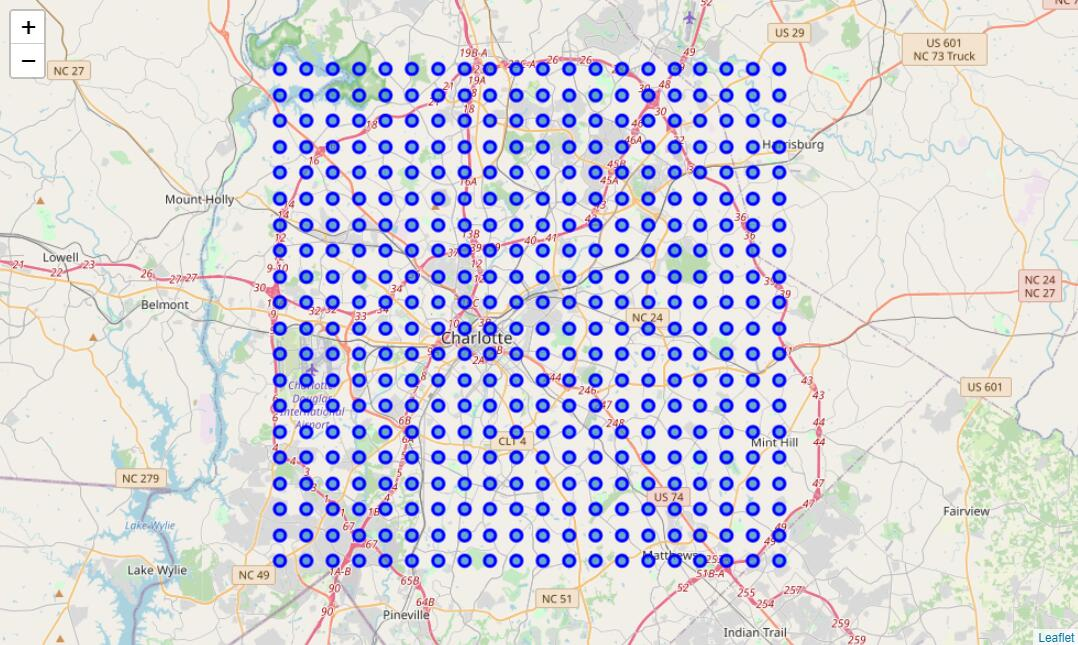
\includegraphics[width=1.0\textwidth]{c3.jpg}
\centering
\end{figure}

Then we loop over those coordinates and find venues within a certain radius of each point. Note that we will make that radius slightly larger than the half-distance of the two diagonal grid points to make sure that no venues are ignored.
In the Charlotte case, the radius is 1500 m.
By taking this approach, there will also have overlapping venues, where the same venues appear in different grid points.
Since the grid points can locate in sparsely populated areas, where the number of venues is tiny, I will ignore them to avoid potential statistical problems. Only grid points with over 15 venues will be appended into the data.

Example venues look like:
\begin{figure}[h!]
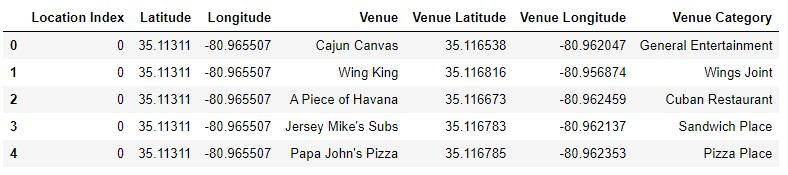
\includegraphics[width=1.0\textwidth]{c4.jpg}
\centering
\end{figure}

In total, 10041 venues are selected. Those data are where we want to get insight from.

Here I show another example to prove the workflow.
Find Atlanta on google map, and select the 
Input point 1 is $33.620260, -84.543165$, point 2 is $34.024354, -84.112095$, and the sample size is 20$\times$20:
\begin{figure}[h!]
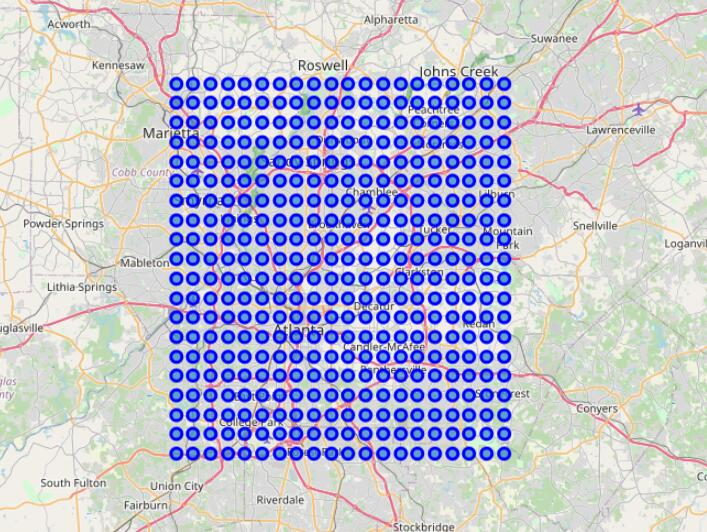
\includegraphics[width=1.0\textwidth]{c5.jpg}
\centering
\end{figure}

\newpage

The data will be grouped by grid point indices and encoded in terms of the venue category. Examples look like:
\begin{figure}[h!]
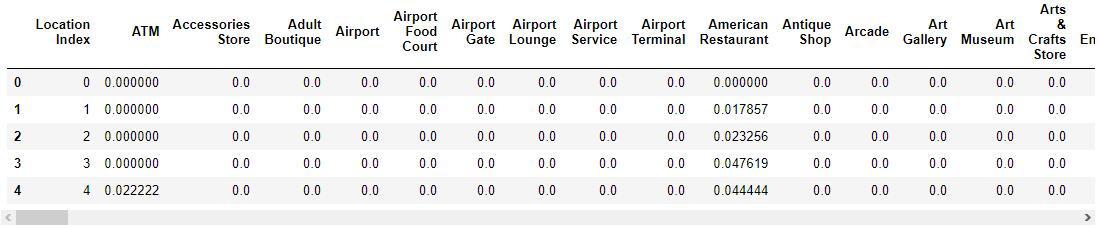
\includegraphics[width=1.0\textwidth]{c6.jpg}
\centering
\end{figure}

Then the data are ready to be analyzed.

\subsection{Usage of the Data}

The most straightforward idea is to use the unsupervised learning techniques only based on the target-city data.
In this case, we do not need data 1.
However, Chinese venues are not typical features for many US cities; it is highly possible that naive unsupervised learning techniques cannot distinguish the Chinese district from other districts.
Therefore, data 1 will play a vital role in screening the venue types and possibly introducing weighted distances during unsupervised learning.

\newpage

\section{Methodology}
\subsection{Naive K-means Clustering}
There are multiple possible approaches to achieve our goal of identifying Chinese districts.
A categorizer using logistic regression or an agglomerated decision tree can do the job with enough data and training.
However, due to the limited Foursquare queries we have access to, unsupervised learning techniques are more suitable for this project since they do not need sizable data sets to train.
K-means clustering algorithm is a clustering algorithm that partition data into k clusters which minimize the in-cluster variance. It starts with a chosen number of "centroids", which are then iteratively optimized to minimize the square sum of distances from in-cluster data points to centroids.\cite{likas2003global}

The first idea that comes to my mind is whether it is possible to directly identify Chinese districts by mixing those Chinatown points into a target city and seeing what clusters they belong to.
Heuristically, A grid point area with venues similar to a classical Chinatown should also be a Chinese district.
I name this approach "Naive K-means".
In this test, I mix the five Chinatown data directly with the 327 grid points (with over 15 venues within that grid) in Charlotte and run K-means clustering with $k=7$.

\begin{figure}[h!]
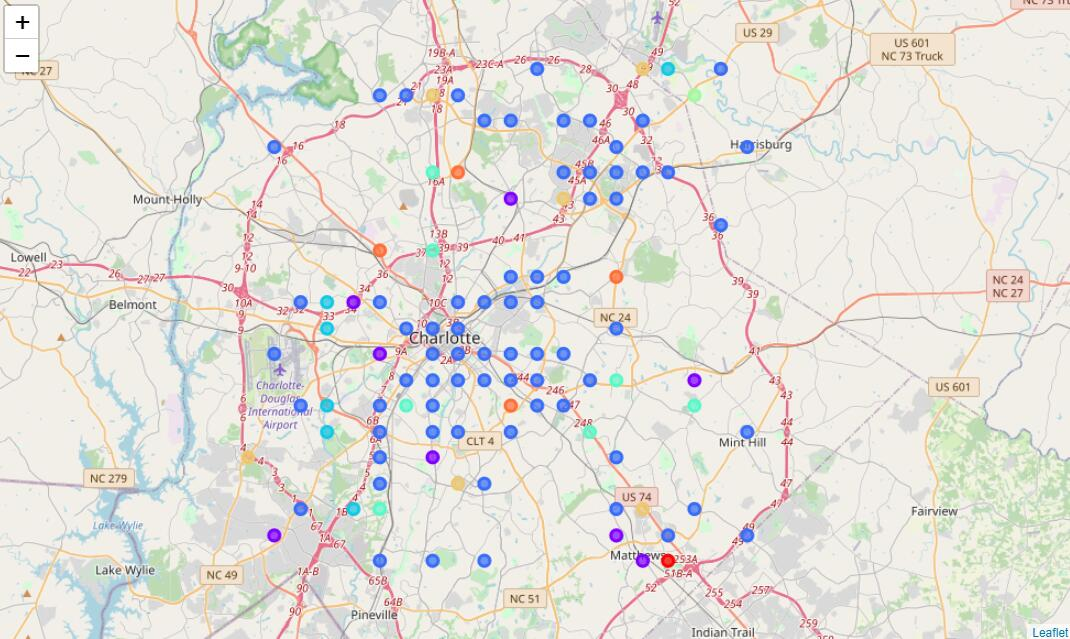
\includegraphics[width=1.0\textwidth]{cn1.jpg}
\centering
\end{figure}

As shown in the figure, the blue points are all in the same cluster as the five Chinatowns.
It is obvious that the algorithm fails to distinguish Chinese districts from regular urban areas.

\newpage

\subsection{Feature Analysis}

Digging into the problem, I group the Chinatown venues and Charlotte grid point venues by venue categories.
Venue categories of the five Chinatown locations:
\begin{figure}[h!]
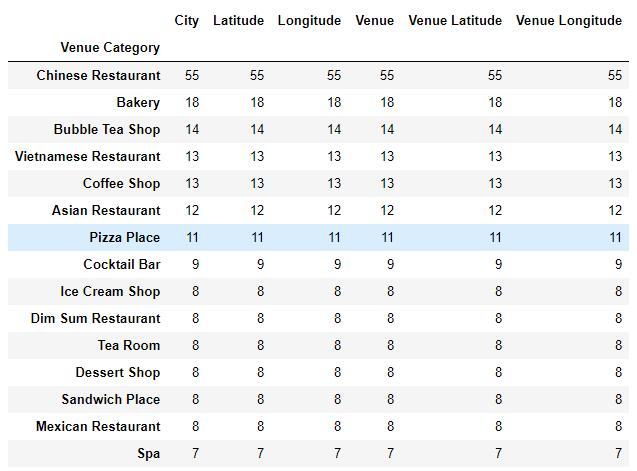
\includegraphics[width=0.7\textwidth]{csp1.jpg}
\centering
\end{figure}
Venue categories of the 400 Charlotte points:
\begin{figure}[h!]
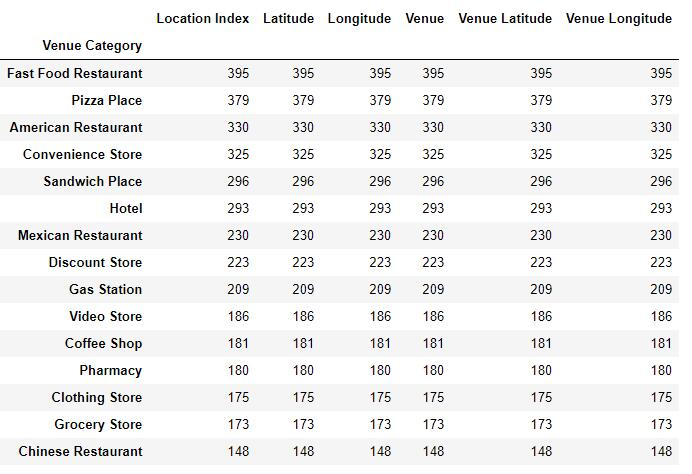
\includegraphics[width=0.7\textwidth]{csp2.jpg}
\centering
\end{figure}
Notice that some frequent venues in the Chinatown locations are also common in Charlotte grid point locations.
Those venue types can be one of the major reasons that the naive K-means put so many points in the same cluster with the Chinatown data.
For example, "pizza place" and "coffee shop" don't look like a feature of a Chinese district from my personal experiences.
However, as for "Bakery", I have no idea whether it is a Chinese district feature.
Therefore, statistical approach should be used to identify useful features.
A venue category frequency is a feature if it is significantly more frequent in a Chinatown than in regular US urban areas.
Since the variance of the venue counts is huge, I use the $1.5 \times IQR$ standard as in-sample testing.
IQR range includes venue frequencies within the $25\%$ to $75\%$ of all sample points.
We sample the 327 Charlotte grid for each venue category and plot their $1.5 \times IQR$ bars. 
If a type of Chinatown venue frequency is higher than that bar, it will be considered a Chinese district feature.

The box plots that show $1.5 \times IQR$ for grid point venue frequencies:
\begin{figure}[h!]
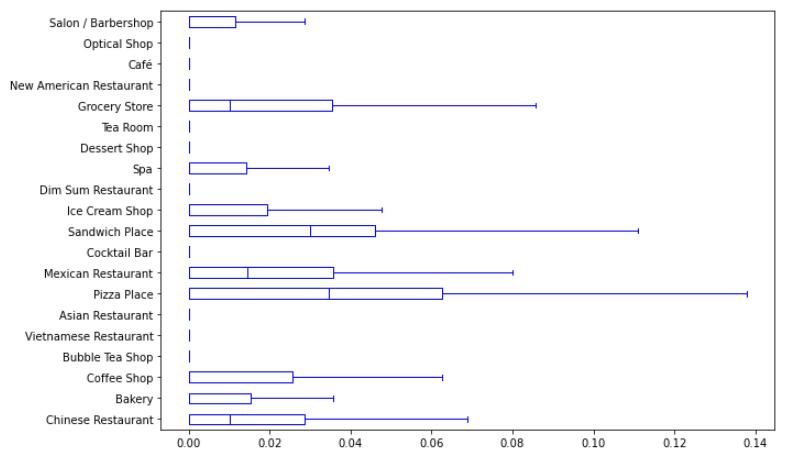
\includegraphics[width=1.0\textwidth]{cn2.jpg}
\centering
\end{figure}
Note that some venue types have $1.5 \times IQR$ bar at 0. It indicates that more than $75\%$ of grid point areas have zero venues of these types.

Then I overlap the Chinatown venue frequencies with this figure:
\begin{figure}[h!]
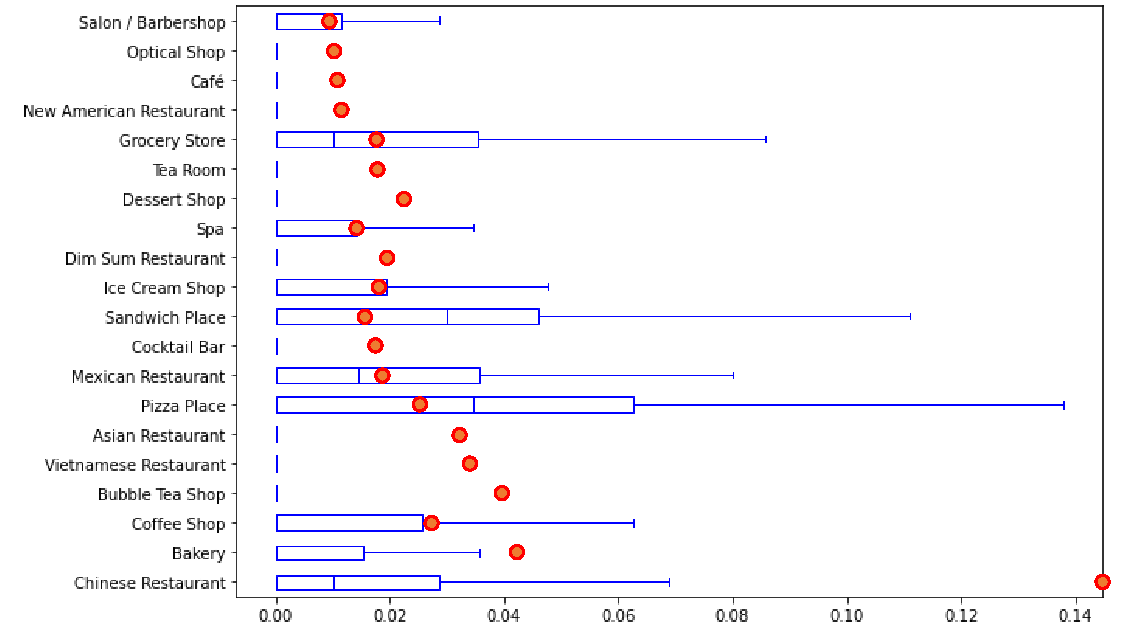
\includegraphics[width=1.0\textwidth]{cn3.pdf}
\centering
\end{figure}
These results clearly show what venue categories are Chinese district features and what is not.
As I expected, "coffee shop" and "pizza place" are not Chinese district features, and "Chinese restaurant" is a Chinese district feature.
Surprisingly, "Bakery" is a feature of Chinese districts, which is different from my expectations.

\newpage

\subsection{Weighted K-means}

With these features in hand, I can exclude the unrelated features to improve the clustering procedure and only keep the related features (noted as $A$).
And we mark the venue frequencies in five Chinatowns as $F_C$ and the 327 grid point sample frequencies as $F_S$.
To further enhance the distinguishing or recognition capability of the clustering procedure, I weighted the frequencies of those related features in Charlotte grid points by multiplying them with the Chinatown frequencies.
$$ F_{S, W} = (F_S \times A) \circ F_C $$
where $\circ$ represents element-wise (Hadamard) product, and $F_{S, W}$ is the weighted venue frequencies ready for the K-means clustering computation.
By this treatment, the venue categories that are more frequent in the Chinatown data (like Chinese restaurants) get more attention and importance during the clustering.
In the following section, I will use this procedure to identify the Chinese district in Charlotte and Atlanta.

\section{Result and Discussion}

\subsection{Results of Charlotte}

\begin{figure}[h!]
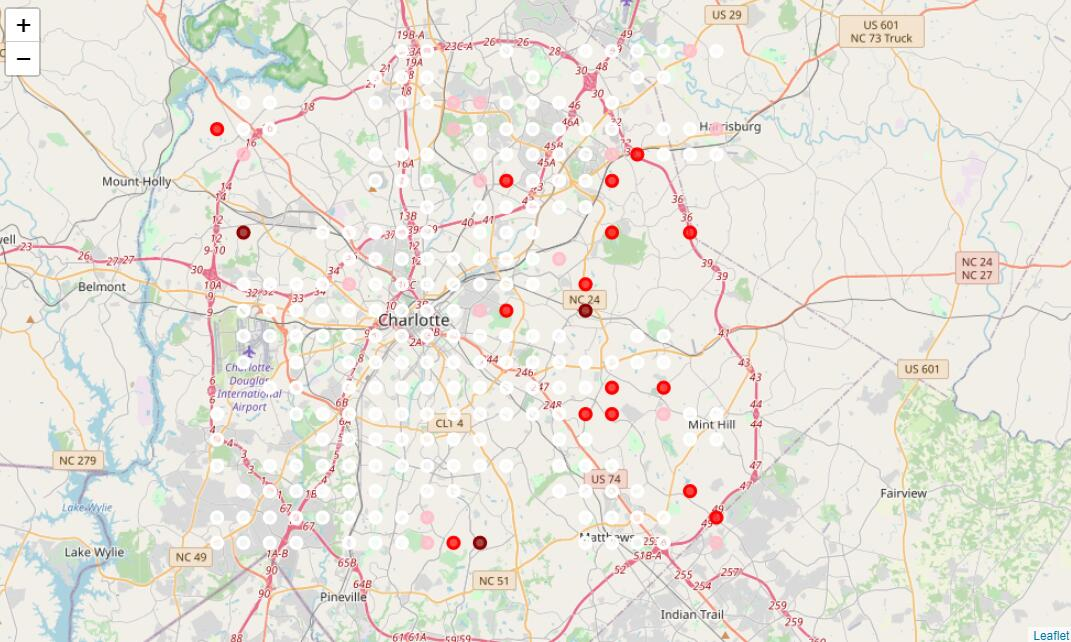
\includegraphics[width=1.0\textwidth]{cn4.jpg}
\centering
\end{figure}

I first apply the weighted K-means clustering on the Charlotte grid points; the figure here shows the result.
There are seven resulting clusters.
To extract the important information, we sort these seven clusters according to the sum of the average frequency in $F_{S, W}$ and color only the top three clusters into deep red, red and pink colors.
The other four clusters will be painted white.
From the results, we can see that Eastern Charlotte, especially areas around NC 24, seems to have more Chinese districts.
We should also notice that the distribution of those red clusters is pretty dispersed.
From those data, it is also possible that Charlotte does not have a major Chinese district like New York or San Francisco, or it may locate somewhere outside of the urban areas.

\subsection{Results of Atlanta}

\begin{figure}[h!]
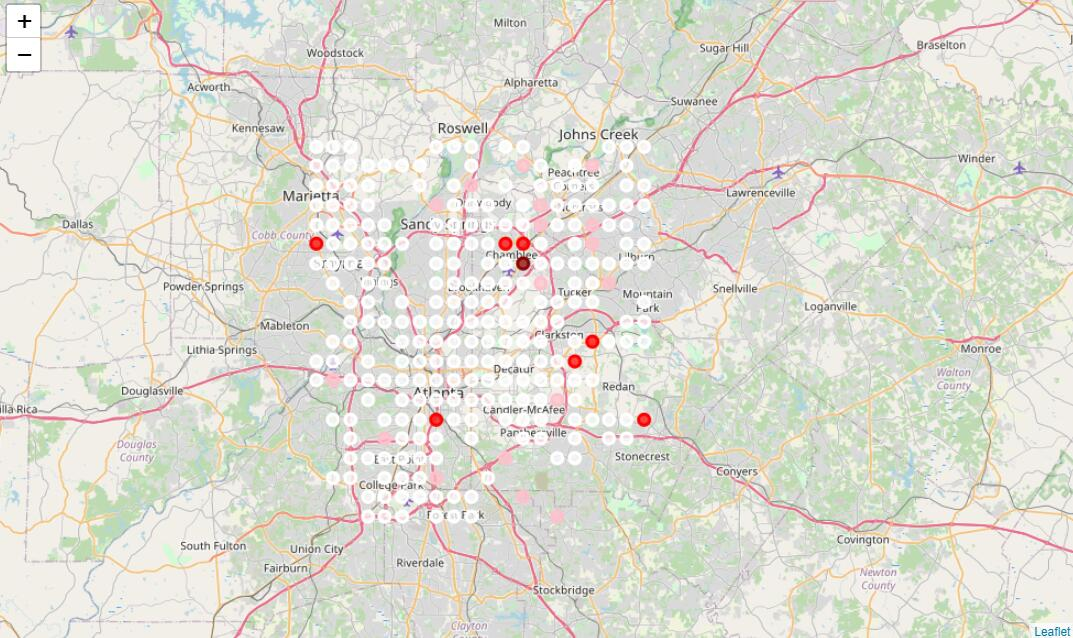
\includegraphics[width=1.0\textwidth]{cn5.jpg}
\centering
\end{figure}

The second city I investigate is Atlanta.
The grid points and results are generated through the same procedure as Charlotte.
After running the weighted K-means clustering, the results show several significant Chinese district possibilities around Chamblee.
This result is consistent with my experiences in Atlanta.
The area around Chamblee is a traditional Chinese district in Atlanta.
It is evident that my procedure successfully captures this information without explicit training.

\newpage

\subsection{Potential Problems and Extensions}
One major limitation to my current procedure is the venue frequency used as distance indicators in clustering.
In Section 4, the weighted K-means clustering algorithm generates seven clusters based on $F_{S, W}$. I sort them according to average $F_{S, W}$ to color them deep red, red, or pink.
This step is a quick-and-dirty trick and is not rigorously justified.
Since different grid point areas have different venue counts, an area with higher "Chinese restaurant" or "Bakery" frequencies is not necessarily a Chinese district.
For example, suppose a grid point area has only 15 venues, and two of them are in the "Chinese restaurant" category. In that case, this point will have a "Chinese restaurant" frequency of 0.133, which boosts their average $F_{S, W}$ significantly.
However, this area might simply be some suburb that happens to have two Chinese venues.

Therefore, a potential improvement to my procedure is to take the total number of venues of each grid points into account to normalize the frequencies.
The other simple solution is to raise the minimum number of venues from 15 to 30 or 50 for each grid point area.

The other concern may be the feature selection in Section 3.2.
The current feature selection sampling is based on the 327 Charlotte grid point samples.
However, each city in the US may have its own unique distribution of venue categories.
For a more compelling and well-supported argument, more samples should be taken.
A possible practice is to sample grid points around our target city, implementing the feature selection in Section 3.2 as part of the pipeline.

\section{Conclusion}
In conclusion, I proposed a procedure to identify Chinese districts in any city.
The procedure utilizes venue frequencies as the indicator to cluster geography grid points around a target city.
Those indicators are selected and weighted based on the venue frequency data from five major Chinatowns in the US.
I apply this procedure to two middle-sized cities in the US. The results are consistent with my personal experiences.
This procedure is still primitive, and further improvement is expected.

\section{Acknowledgement}
This project is a part of my "IBM Data Science Professional Certificate" assignment.

\newpage

\bibliographystyle{unsrt}
\bibliography{capstone}

\end{document}
